%%%%%%%%%%%%%%%%%%%%%%%%%%%%%%%%%%%%%%%%%
% University/School Laboratory Report
% LaTeX Template
% Version 3.1 (25/3/14)
%
% This template has been downloaded from:
% http://www.LaTeXTemplates.com
%
% Original author:
% Linux and Unix Users Group at Virginia Tech Wiki 
% (https://vtluug.org/wiki/Example_LaTeX_chem_lab_report)
%
% License:
% CC BY-NC-SA 3.0 (http://creativecommons.org/licenses/by-nc-sa/3.0/)
%
%%%%%%%%%%%%%%%%%%%%%%%%%%%%%%%%%%%%%%%%%

%----------------------------------------------------------------------------------------
%	PACKAGES AND DOCUMENT CONFIGURATIONS
%----------------------------------------------------------------------------------------

\documentclass[a4paper,12pt,notitlepage]{report}

\usepackage[version=3]{mhchem} % Package for chemical equation typesetting
\usepackage{siunitx} % Provides the \SI{}{} and \si{} command for typesetting SI units
\usepackage{graphicx} % Required for the inclusion of images
\usepackage{natbib} % Required to change bibliography style to APA
\usepackage{amsmath} % Required for some math elements 
\usepackage[utf8]{inputenc}
\usepackage[T1]{fontenc}
\usepackage{titlesec, blindtext, color}
\definecolor{gray75}{gray}{0.75}
\newcommand{\hsp}{\hspace{20pt}}
\titleformat{\chapter}[hang]{\Huge\bfseries}{\thechapter\hsp\textcolor{gray75}{|}\hsp}{0pt}{\Huge\bfseries}
[
\vspace{-2ex}
\textcolor{gray75}{\rule{\textwidth}{0.3pt}}
]

\titleformat{\section}[hang]{\Large\bfseries}{\thesection\hsp\textcolor{gray75}{|}\hsp}{0pt}{\Large\bfseries}

\setlength\parindent{0pt} % Removes all indentation from paragraphs

\renewcommand{\labelenumi}{\alph{enumi}.} % Make numbering in the enumerate environment by letter rather than number (e.g. section 6)

\newcommand{\HRule}{\rule{\linewidth}{0.5mm}}
%\usepackage{times} % Uncomment to use the Times New Roman font


%----------------------------------------------------------------------------------------
%	DOCUMENT INFORMATION
%----------------------------------------------------------------------------------------

\title{ \huge \bfseries Computer Graphics \\ \Large DTU 02561 (fall 2014) \\ REPORT } % Title
\author{Karol \textsc{Dzitkowski} s142246} % Author name
\date{\today} % Date for the report

\begin{document}

\maketitle % Insert the title, author and date
\HRule \\[1.5cm]
\begin{figure}[b]
	\begin{center}
		
\includegraphics{DTU-logo}
	\end{center}
\end{figure}

\clearpage

\tableofcontents
\clearpage

% If you wish to include an abstract, uncomment the lines below
% \begin{abstract}
% Abstract text
% \end{abstract}

%----------------------------------------------------------------------------------------
%	CONTENT
%----------------------------------------------------------------------------------------

\chapter{Exercise 1}
The purpose of this exercise is to give a short introduction to
create, edit, link and run C/C++ programs that are based on the
graphics library OpenGL, and the utility libraries Angel and
GLUT.
\section{Part 1}
I drew another triangle by adding extra 3 vertices to the vertexData array:
\begin{figure}[ht!]
	\begin{center}
		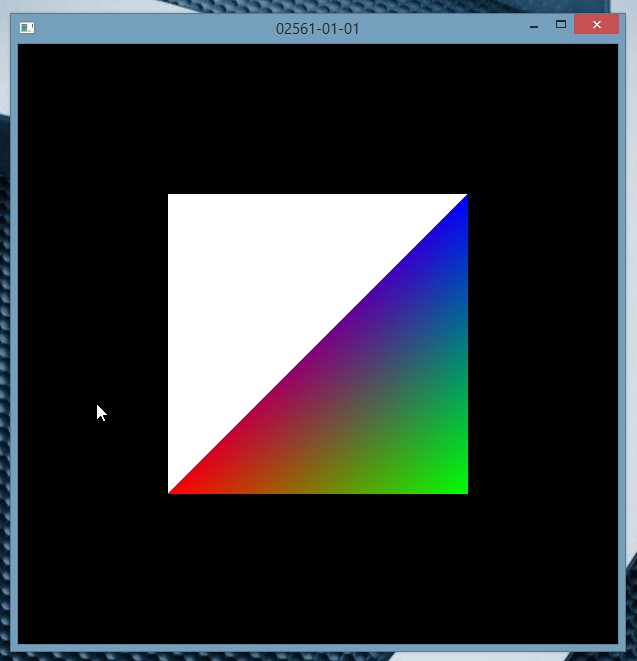
\includegraphics[width=0.5\textwidth]{figures/exercise_1_part_1}
	\end{center}
	\caption{Exercise 1 part 1 output}
\end{figure} \\
Below I described a meaning of each function used in a program:
\begin{description}
	\item[glGetAttribLocation] -- Returns the location of an attribute variable
	\item[glClearColor] -- specify clear values for the color buffers
	\item[glClear] -- clear buffers to preset values
	\item[glUseProgram] -- Installs a program object as part of current rendering state
	\item[glBindVertexArray] -- binds the vertex array object with name
	\item[glDrawArrays] -- render primitives from array data
	\item[glutSwapBuffers] -- swaps the buffers of the current window if double buffered
	\item[glViewport] -- sets the viewport
	\item[glGenVertexArrays] -- generate vertex array object names
	\item[glGenBuffers] -- generate buffer object names
	\item[glBindBuffer] -- bind a named buffer object
	\item[glBufferData] -- creates and initializes a buffer object's data store
	\item[glVertexAttribPointer] -- specify the location and data format of the array of generic vertex attributes at
	index index to use when rendering
	\item[Angel::InitShader] -- initializes shader programs stored in files passed as attributes
	\item[glutInit] -- initializes the GLUT library
	\item[glutInitContextVersion] -- sets openGL version we use
	\item[glutInitContextFlags] -- sets flags in GLUT library
	\item[glutInitContextProfile] -- sets profile of GLUT library
	\item[glutInitDisplayMode] -- sets the initial display mode
	\item[glutCreateWindow] -- creates a top-level window with a name passed as argument.
	\item[glutDisplayFunc] -- sets the display callback for the current window
	\item[glutReshapeFunc] -- sets the reshape callback for the current window
	\item[glutReshapeWindow] -- sets the window width and height
	\item[Angel::InitOpenGL] -- initializes OpenGL
	\item[glutMainLoop] -- enters the GLUT event processing loop
\end{description}


\section{Part 2}
I extended the program to include a triangle and rotated a rectangle using code below:
\begin{lstlisting}[language=cpp, caption={Exercise 1 part 1 code changes}]
void loadGeometry(){
// add a triangle
Vertex triangleData[triangleSize] = {
	{ vec2(2,2), vec3(1.0, 0.0, 0.0) },
	{ vec2(5,2), vec3(0.0, 1.0, 0.0) },
	{ vec2(3.5,5), vec3(0.0, 0.0, 1.0) }};
triangleVertexArrayBuffer = loadBufferData(triangleData, triangleSize);}

void display(){
// to rotate rectangle
mat4 modelView2 = Angel::RotateZ(45);
glUniformMatrix4fv(modelViewUniform, 1, GL_TRUE, modelView2);
// transform and render the triangle
mat4 modelView;
modelView[0][3]=6;
modelView[1][3]=7;
modelView[2][3]=0;
glUniformMatrix4fv(modelViewUniform, 1, GL_TRUE, modelView);
glBindVertexArray(triangleVertexArrayBuffer);
glDrawArrays(GL_TRIANGLE_FAN, 0, triangleSize);}
\end{lstlisting}
After applying these changes I got an output: \\
\begin{figure}[ht!]
	\begin{center}
		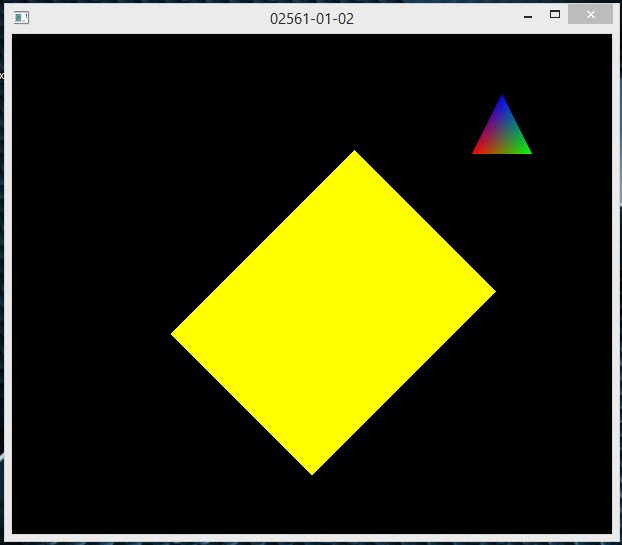
\includegraphics[width=0.45\textwidth]{figures/exercise_1_part_2}
	\end{center}
	\caption{Exercise 1 part 2 output}
\end{figure}


\section{Part 3}
\subsection{glDrawArrays vs glDrawElements}
The nvidia docs say that glDrawElements is faster because of potential vertex sharing.
Function glDrawArrays submits the vertices in linear order, as they are stored in the vertex arrays.
With glDrawElements one has to supply an index buffer. Indices allow to submit the vertices in any 
order, and to reuse vertices that are shared between triangles.
\subsection{Triangle rendering types}
\begin{description}
	\item[GL\_TRIANGLES] - A triangle is composed from every three vertices. First is composed 
	from vertives $(0,1,2)$ second from $(3,4,5)$ and so on. 
	\item[GL\_TRIANGLE\_STRIP] - Draws a series of triangles using vertices $(0,1,2)$ then $(2,1,3)$ then
	$(2,3,4)$ and so on. The ordering is to ensure that the triangles are all drawn with the same
	orientation so that the strip can correctly form part of a surface.
	\item[GL\_TRIANGLE\_FAN] - The first vertex is always held fixed. From there on, every group of
	2 adjacent vertices form a triangle with the first.
\end{description}
\subsection{Extended program}
Below I present an output of the extended program:
\begin{figure}[ht!]
	\begin{center}
		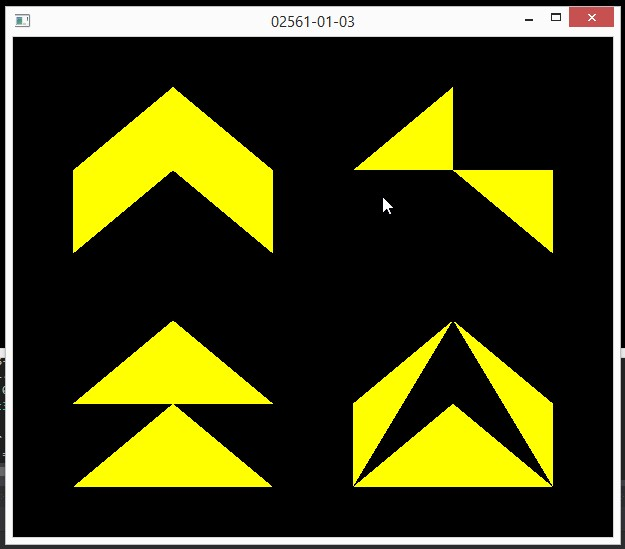
\includegraphics[width=0.45\textwidth]{figures/exercise_1_part_3}
	\end{center}
	\caption{Exercise 1 part 3 output}
\end{figure} 
\clearpage


\section{Part 4}
The resulting screenshot of program extension can be seen in Figure \ref{fig:exercise_1_part_4} \\
\begin{figure}[ht!]
	\begin{center}
		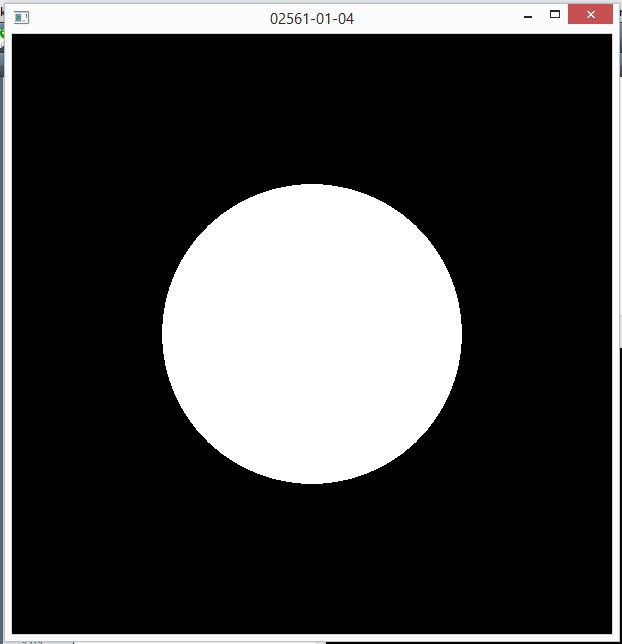
\includegraphics[width=0.5\textwidth]{figures/exercise_1_part_4}
	\end{center}
	\caption{Exercise 1 part 4 output}
	\label{fig:exercise_1_part_4} 
\end{figure} \\
I did it using GL\_TRIANGLE\_FAN option in glDrawArrays and created vertices in vertexData using code:
\begin{lstlisting}[language=cpp, caption={Exercise 1 part 4 creating circle vertices}]
void loadBufferData() {
	for (int i=1; i < NUMBER_OF_VERTICES; i++)
	{
		float const t = 2*M_PI*(float)i/(float)(NUMBER_OF_VERTICES - 2);
		vertexData[i].x = origin.x + cos(t)*CIRCLE_RADIUS;
		vertexData[i].y = origin.y + sin(t)*CIRCLE_RADIUS; 
	}
	//...
}
\end{lstlisting}
\clearpage
\section{Part 5}
I succeeded to draw the figure by using scaling, rotation and transforming from Angel library and
glDrawArrays function with GL\_TRIANGLES option.
For example printing inside triangles is done using code:
\begin{lstlisting}[language=cpp, caption={Exercise 1 part 5 inside triangles}]
mat4 innerTriangleModelView = Angel::Scale(10,10,10);
innerTriangleModelView *= Angel::RotateX(180);

for(int i=0; i<4; i++)
{
	glUniformMatrix4fv(modelViewUniform, 1, GL_TRUE, innerTriangleModelView);
	glDrawArrays(GL_TRIANGLES, 0, NUMBER_OF_VERTICES);
	innerTriangleModelView *= Angel::RotateZ(90);
}
\end{lstlisting}
\begin{figure}[ht!]
	\begin{center}
		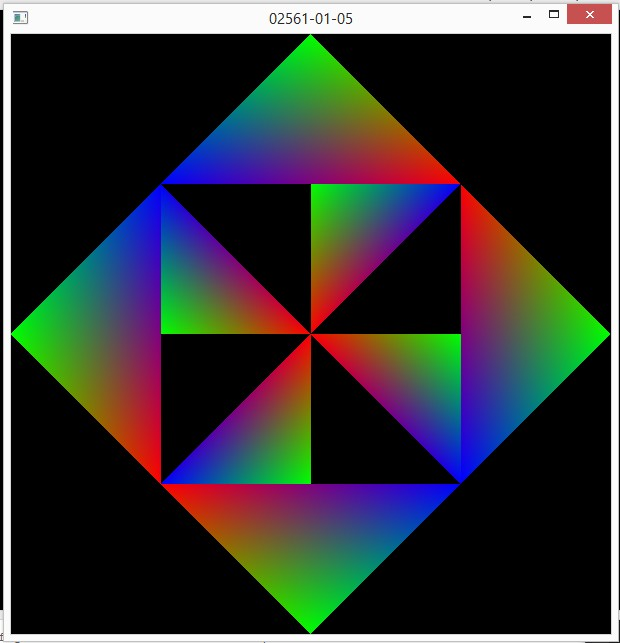
\includegraphics[width=0.5\textwidth]{figures/exercise_1_part_5}
	\end{center}
	\caption{Exercise 1 part 5 output}
	\label{fig:exercise_1_part_5} 
\end{figure}
\clearpage

\section{Part 6}
Transformation matrix which maps a point $(xw,yw)$ to the point $(xv,yv)$ considering a
window - viewport pair as 
$$
w = [w_{x_{min}},w_{x_{max}},w_{y_{min}},w_{y_{max}}],
v = [v_{x_{min}},v_{x_{max}},v_{y_{min}},v_{y_{max}}]
$$
looks like that:
\begin{align*}
M_{wv} =
  \begin{bmatrix}
    \dfrac{v_{x_{max}} - v_{x_{min}}}{w_{x_{max}} - w_{x_{min}}} & 0 & v_{x_{min}}
    - w_{x_{min}} \cdot \dfrac{v_{x_{max}} - v_{x_{min}}}{w_{x_{max}} - w_{x_{min}}} \\
    0 & \dfrac{v_{y_{max}} - v_{y_{min}}}{w_{y_{max}} - w_{y_{min}}} & v_{y_{min}}
    - w_{y_{min}} \cdot \dfrac{v_{y_{max}} - v_{y_{min}}}{w_{y_{max}} - w_{y_{min}}} \\
    0 & 0 & 1
  \end{bmatrix}
\end{align*}

And is a concatenation of three transformations:
$$
M_{wv} = T_{1}(v_{x_{min}},v_{y_{min}}) \cdot S(s_x, s_y) \cdot T_{2}(w_{x_{min}}, w_{y_{min}})
$$
\begin{itemize}
	\item Translation
		\begin{align*}
		T_{1} =
      \begin{bmatrix}
          1 & 0 & v_{x_{min}} \\
          0 & 1 & v_{y_{min}} \\
          0 & 0 & 1
      \end{bmatrix} 
		\end{align*}
	\item Scaling
		\begin{align*}
    	S =
      \begin{bmatrix}
          \dfrac{v_{x_{max}} - v_{x_{min}}}{w_{x_{max}} - w_{x_{min}}} & 0 & 0 \\
          0 & \dfrac{v_{y_{max}} - v_{y_{min}}}{w_{y_{max}} - w_{y_{min}}} &  0 \\
          0 & 0 & 1
      \end{bmatrix} 
		\end{align*}
	\item Translation
		\begin{align*}
    	T_{2} =
      \begin{bmatrix}
          1 & 0 & -w_{x_{min}} \\
          0 & 1 & -w_{y_{min}} \\
          0 & 0 & 1
        \end{bmatrix} 
		\end{align*}
\end{itemize}
Multiplication of these 3 transformation matrices gives the window-viewport transformation matrix.
In OpenGL glViewport() command is used to define the rectangle of the rendering area where the
final image is mapped.
\clearpage

\section{Part 7}
I rendered a Sierpinski carpet using a recursive function I wrote, below is an output for 6 iterations:
\begin{figure}[ht!]
	\begin{center}
		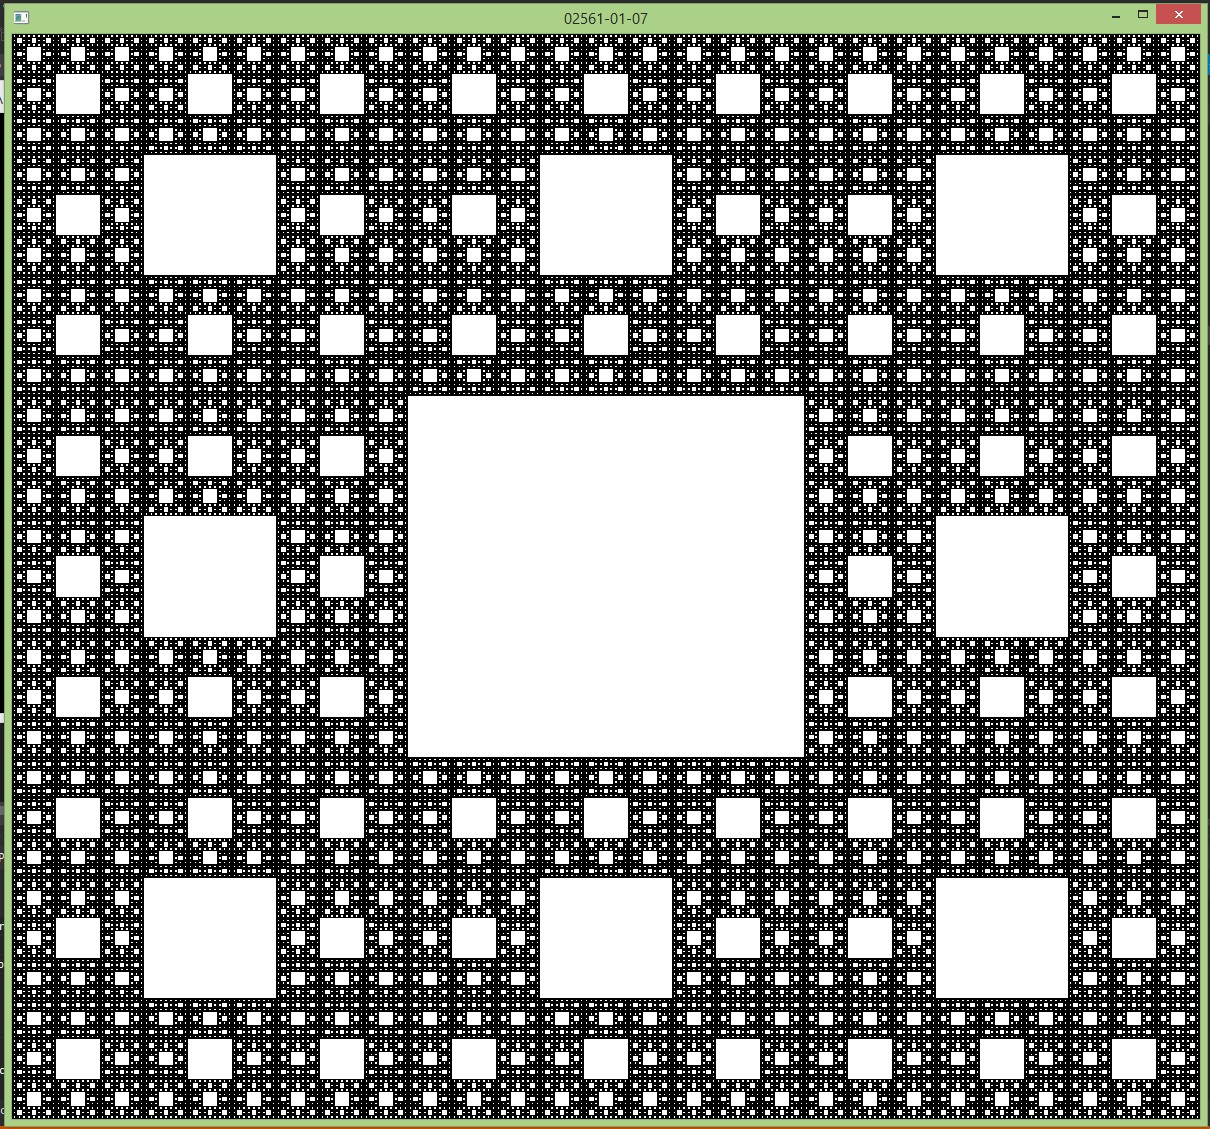
\includegraphics[width=0.5\textwidth]{figures/exercise_1_part_7}
	\end{center}
	\vspace{-4.5ex}\caption{Exercise 1 part 7 output}
	\label{fig:exercise_1_part_7} 
\end{figure} \\
As an input the function which generates points takes vertives of the biggest square. We will also get
an interesting fractal when we switch the order of the vertices (Figure \ref{fig:exercise_1_part_7_extra}).
\begin{lstlisting}[language=cpp, caption={Exercise 1 part 7 point gen.}]
vec2 vertices[4] = {vec2(-1.0, -1.0), vec2(-1.0, 1.0), vec2(1.0, -1.0), vec2(1.0, 1.0)};
divide_square(vertices[0], vertices[1], vertices[2], vertices[3], NumTimesToSubdivide);
\end{lstlisting}
\begin{figure}[ht!]
	\begin{center}
		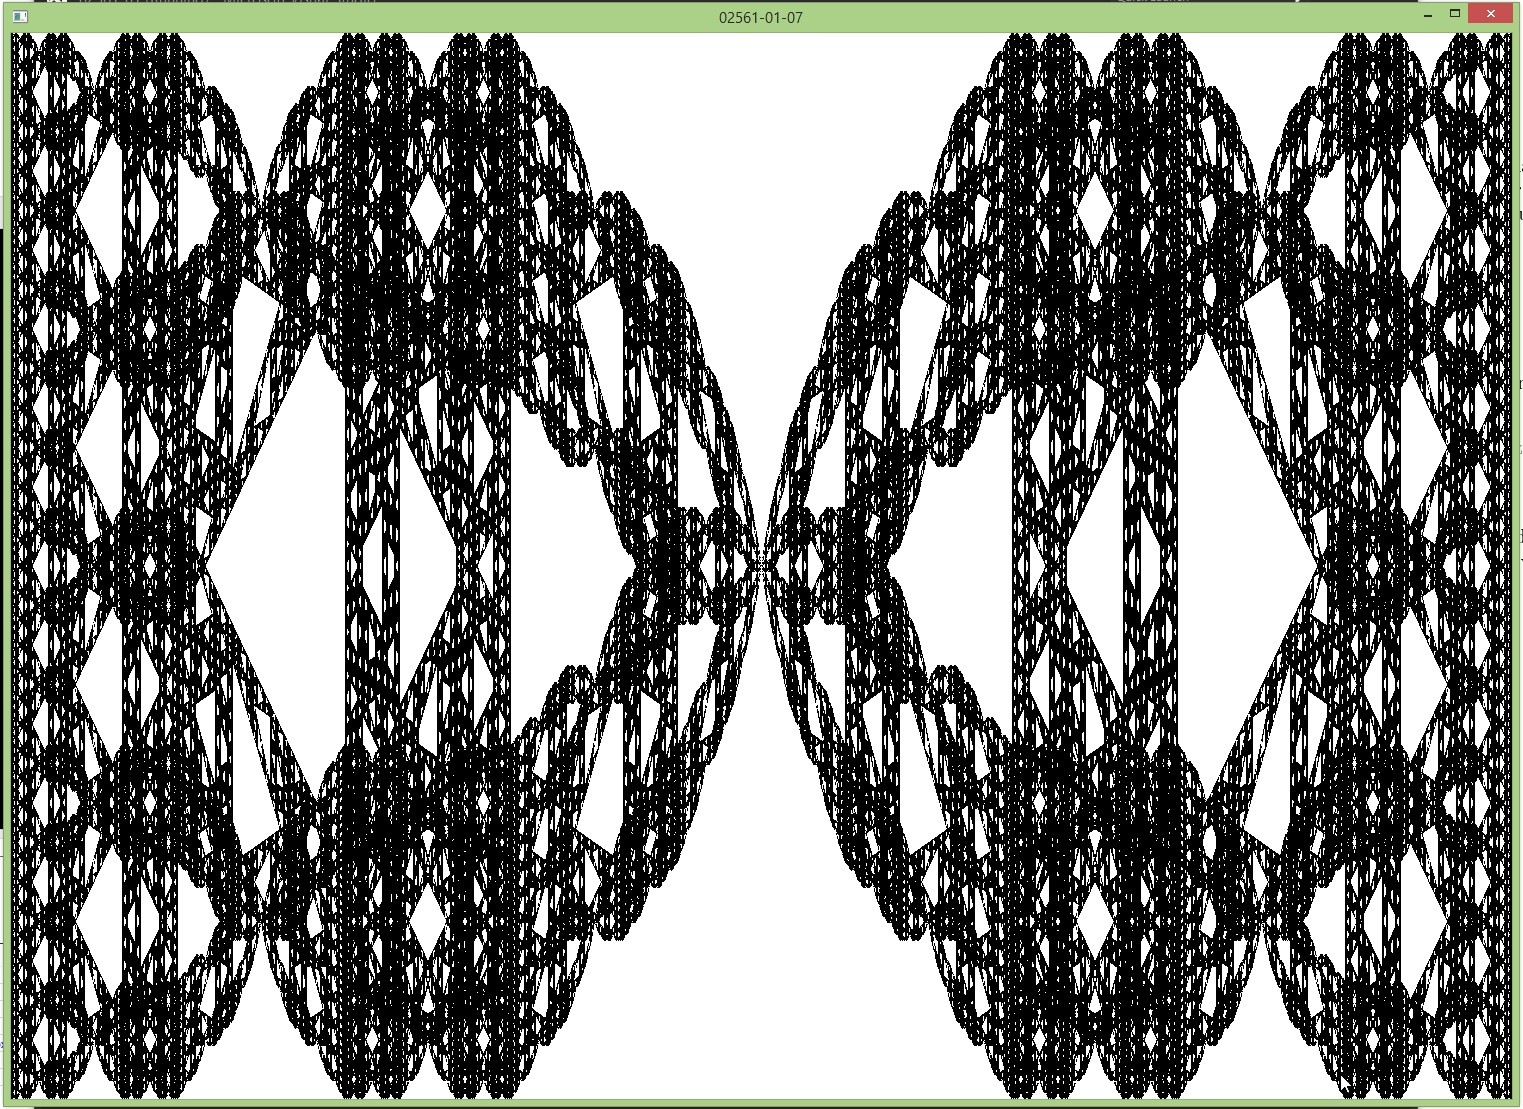
\includegraphics[width=0.5\textwidth]{figures/exercise_1_part_7_extra}
	\end{center}
	\vspace{-4.5ex}\caption{Exercise 1 part 7 output (vertices order changed)}
	\label{fig:exercise_1_part_7_extra} 
\end{figure}

%----------------------------------------------------------------------------------------
%	BIBLIOGRAPHY
%----------------------------------------------------------------------------------------

\bibliographystyle{apalike}
\nocite{*}
\bibliography{references}

%----------------------------------------------------------------------------------------


\end{document}